% Generated by plsimcount.pffigure -- do not edit; regenerate instead.
% figure: A-com-by-order -- Suzuki formulas of each order, r from: Commutator bound (2018)
% source: results/pf-thesis/results.json
% metric=t gatebase=ct merged
% seed=1 t=n template=simcount synth=pygridsynth
% git_commit=c237fe494a6c663dd73df63b2b3fbb5e397a506e git_dirty=False
% source_sha256=6e8b2641428f03f62fe1dfd44b32f3373e9b382199e065d6a7d7340c7875a117
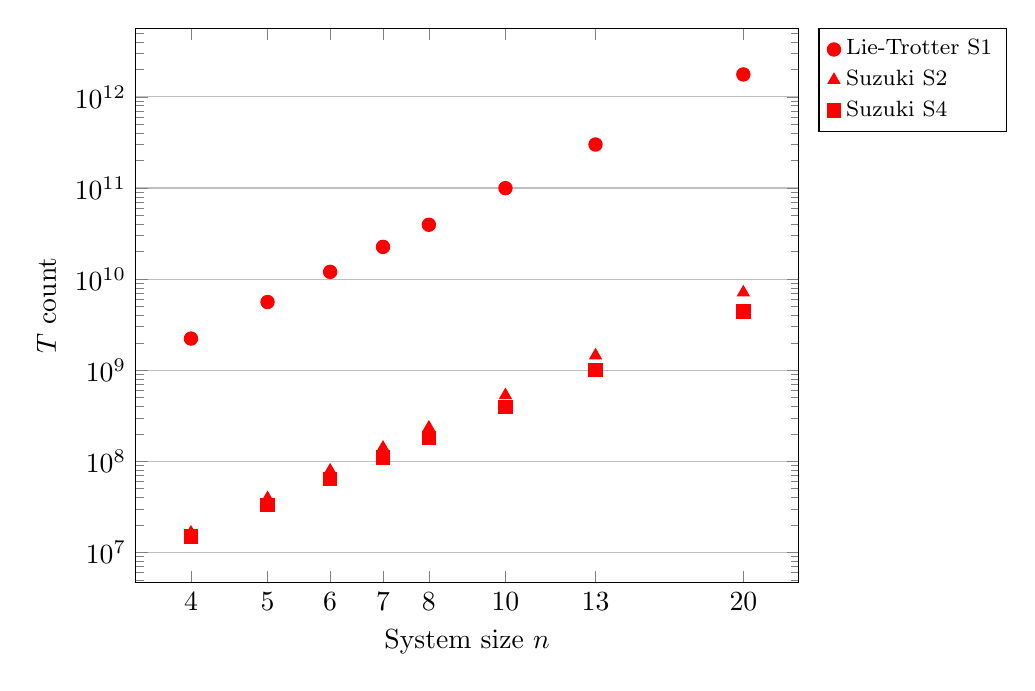
\begin{tikzpicture}
  \begin{loglogaxis}[
    width=10cm,
    xlabel={System size $n$},
    ylabel={$T$ count},
    xtick={4,5,6,7,8,10,13,20},
    xticklabels={4,5,6,7,8,10,13,20},
    ymajorgrids=true,
    legend pos=outer north east,
    legend cell align=left,
    legend style={font=\footnotesize},
  ]
    \addplot[only marks, red, mark=*, mark size=2.4pt, mark options={solid, fill=red}] coordinates {
      (4,2224878106)
      (5,5605598614)
      (6,12019522502)
      (7,22585529744)
      (8,39551101166)
      (10,99690635856)
      (13,300317990958)
      (20,1765948340376)
    };
    \addlegendentry{Lie-Trotter S1}
    \addplot[only marks, red, mark=triangle*, mark size=2.4pt, mark options={solid, fill=red}] coordinates {
      (4,16478640)
      (5,39306456)
      (6,79095600)
      (7,140949800)
      (8,233847800)
      (10,530870754)
      (13,1450201024)
      (20,7125229868)
    };
    \addlegendentry{Suzuki S2}
    \addplot[only marks, red, mark=square*, mark size=2.4pt, mark options={solid, fill=red}] coordinates {
      (4,14915200)
      (5,32951920)
      (6,64395408)
      (7,109841564)
      (8,179440360)
      (10,396662514)
      (13,1006735608)
      (20,4420711640)
    };
    \addlegendentry{Suzuki S4}
  \end{loglogaxis}
\end{tikzpicture}
